\chapter{Introduction}\label{Ch:Intro}
When we open the history book of the universe, we find blank pages in the middle. These blank pages correspond to periods in cosmic history where we have no direct data. One such time period is the $''$Dark Ages$''$ ($z \sim 1100$ to $z \sim 30$), which started when light and matter decoupled during recombination and ended with the births of the first stars in the universe. Following that came the $''$Cosmic Dawn$''$ ($z\sim 30$ to $z\sim 10$), when the first stars lived, died and impacted the universe around them. Very little is known about these times; as no one has been able to observe them directly. 

Recently, the development of \cm cosmology has provided a potential tool for measuring these eras of our history and filling in some of the blanks. There are a number of experiments that seek to utilize this tool to study the universe. Many of the experiments are interested in the Dark Ages, Cosmic Dawn, or the Epoch of Reionization that immediately follows them.  

\section{Hydrogen \cm Signal}
In order to discuss \cm cosmology, we first need to understand the basic physics behind the signals that we are studying. There are four components that need to be defined to facilitate this understanding. First, we need to review the atomic states of hydrogen and in particular the hyperfine splitting of the ground state. Second, we need to define the spin temperature of a cloud of neutral hydrogen atoms and discuss how emission and absorption change the spin temperature. Third, we need to define brightness temperature and detail how that temperature can change when it passes through a cloud of hydrogen gas. Fourth, we need to combine spin temperature and brightness temperature via the opacity of a cloud of hydrogen gas. 

\subsection{Hydrogen Atomic States}
To understand the \cm signal, we start with the structure of the hydrogen atom; one proton and one electron. The proton and electron each have a spin $\pm \frac{1}{2}$, which leads to a splitting of the ground state of hydrogen depending on the total spin angular momentum of the atom. The energy of the atom is lower when the spins are anti-aligned and the total spin angular momentum of the atom is zero than when the spins are aligned with a total spin angular momentum of one. This energy difference is called $''$hyperfine$''$ splitting; with the spin 0 state being a singlet and the spin 1 state being a triplet (and therefore three times more likely). The energy difference from this splitting is $h \nu_{10}$, where $\nu_{10}=1420.405$ MHz and $\lambda_{10} =  21$ centimeters.  

\subsection{Spin Temperature}
When working with a cloud of hydrogen atoms rather than a single atom, we need to compare the number of atoms in the two states within the cloud. To do this, we define the spin temperature using Boltzmann's law for a cloud in thermodynamic equilibrium. A spin temperature (\ts) is defined with the ratio of the the two states $n_1/n_0$. 

\begin{equation}\label{Eq:T_s}
\frac{n_1}{n_0} \equiv 3 e^{- h \nu_{10} / kT_S} = 3 e^{-T_*/T_S}
\end{equation} 

\subsection{Changing the Spin Temperature} \label{Sec:dT_S}
Change of the spin temperature occurs through emission and absorption of \cm photons corresponding to a transition between the two spin states. Transitions occur when the atom either spontaneously emits a photon or is induced to emit or absorb a photon due to external forces. These transitions can be described using a differential equation (Equation \ref{Eq:dn}), and each type of transition (m) has a different $X^m_{ij}$. 

\begin{equation} \label{Eq:dn}
\Big( \frac{d n_i}{dt} \Big)_m = X^m_{ij} n_i
\end{equation}

If the cloud is in equilibrium, the rates of change are set such that $n_{total} = n_0 + n_1$ is a constant. This means that $d n_0/dt = d n_1 /dt$, allowing us to calculate the spin temperature using Equation \ref{Eq:sn} at any time.

\begin{equation} \label{Eq:sn}
n_0 \sum^m X^m_{01} = n_1 \sum^m X^m_{10}
\end{equation}

\subsubsection{Spontaneous Emission}
Spontaneous emission due to a transition between the spin states caused by quantum interactions with the electromagnetic environment. Because the spin transition is a forbidden one, the lifetime of the higher energy (triplet) state is over 10 million years. The exact rate is set by the Einstein A coefficient ($A_{10}$), which is defined as: 

\begin{equation}
A_{10} = \frac{64 \pi^4 \beta^2}{3 h \lambda^3} = 2.85 x 10^{-15} sec^{-1}
\end{equation}

where $\beta$ is the Bohr magneton. The small magnitude of $A_{10}$ means that spontaneous emission of \cm photons is very rare. 

\subsubsection{Absorption and Stimulated Emission}
In comparison to spontaneous emission, both absorption and stimulated emission are caused by external mechanisms and can therefore occur much more frequently than spontaneous emission. In the types of hydrogen gas clouds that we are considering, there are only three types of external mechanisms that provide high transition rates. 

\paragraph{Radiation}
The first transition mechanism is caused by incident radiation from an external source of \cm photons such as Cosmic Microwave Background (CMB) photons. The coefficients for this source are $X^R_{01} = B_{01} I_\nu$ and $X^R_{10} = B_{10} I_\nu $, which are the Einstein B coefficients and can be related to $A_{10}$ by Equation \ref{Eq:Bxx}. 

\begin{equation} \label{Eq:Bxx}
B_{01} I_{\nu} = 3 B_{10} I_{\nu} = 3 A_{10} \Big( \frac{\lambda^2 I_\nu}{ 2 h \nu_{10}} \Big)
\end{equation}

\paragraph{Collisions}
The second transition mechanism is collisions between the atoms and electrons in a hydrogen gas cloud. This mechanism has coefficients $C_{01}$ and $C_{10}$. Because the system is in thermodynamic equilibrium, we can define a kinetic temperature (\tk) using the transition coefficients. 

\begin{equation}
\frac{C_{01}}{C_{10}} \equiv 3 e^{-T_*/T_K}
\end{equation}

\paragraph{Light}
The third and final mechanism is photons of light at other wavelengths causing changes to the atoms. This is known as the Wouthuysen-Field mechanism \cite{wouthuysen_1952}\cite{field_1958} and will be discussed in greater detail in Section \ref{Sec:WFM}. For now, we'll just define a light temperature ($T_L$) using the same form as the other temperatures.

\begin{equation}
\frac{L_{01}}{L_{10}} = 3 e^{-T_*/T_L}
\end{equation}

\subsubsection{Spin Transition Rate Equation}
When we combine all of these sources of transitions using Equation \ref{Eq:sn}, we can derive an equation for \ts. We start with the summations, as shown in Equation \ref{Eq:sns}.  

\begin{equation}\label{Eq:sns}
n_1(A_{10} + B_{10} I_\nu + C_{10} + L_{10}) = n_0 (B_{01} I_\nu + C_{01} + L_{01})
\end{equation}

By rearranging and substituting in Equation \ref{Eq:T_s}, we get a direct relationship between the transition rates and the spin temperature. 

\begin{equation}
\frac{n_1}{n_0} = 3 e^{-T_*/T_S} = \frac{B_{01} I_\nu + C_{01}+ L_{01}}{A_{10}+ B_{10} I_\nu + C_{10} +L_{10}}
\end{equation}

Since $T_* = 68.1 mK$ and $T_S \gg T_*$, we can approximate the exponentials ($e^{-T_*/T} \simeq 1-T_*/T$) and rearrange to get:

\begin{equation}\label{Eq:dT_s}
T_s = \frac{T_{R} + x_K T_{K} + x_{L} T_{L}}{1+x_K +x_{L}}
\end{equation}

where the coupling coefficients are $x_K = T_* C_{10}/A_{10} T_K$ and $x_L = T_* L_{10} / A_{10} T_L$, and $T_R$ is the incident radiation temperature. 

\subsection{Brightness Temperature}
The primary sources of incident radiation for hydrogen gas clouds are blackbody sources such as the CMB. These blackbody sources have a spectral energy distribution ($B_\nu (T)$) defined by the Planck spectrum:

\begin{equation}
I_{\nu} (T) = B_{\nu}(T) = \frac{ 2 h \nu^3 / c^2}{e^{h \nu / k T}-1}
\end{equation}

For long wavelengths, we use the Rayleigh-Jeans approximation ($B_{\nu} (T) \simeq (2 k \nu^2 / c^2) T$) to give us a brightness temperature ($T_b (\nu)$) \cite{carroll2007}. 

\subsubsection{Change in Brightness Temperature}
Now, brightness temperature will change as the light travels through the universe. Such change can be caused by the expansion of the universe or by external sources such as passage through gas clouds. 

Expansion of the universe simply causes the brightness temperature at each frequency to decrease at a rate $\propto 1/(1+z)$. 

In comparison, when the light passes through a gas cloud the rate at which the brightness temperature changes varies between frequencies. This rate of change is represented mathematically as a cloud opacity (\tu). Using opacity allows us to write the brightness temperature after passing through the cloud using Equation \ref{Eq:T_bf}. 

\begin{equation}\label{Eq:T_bf}
(T_b (\nu))_{final}= T_{C} (\nu) (1-e^{-\tau_\nu}) +T_{R} e^{-\tau_\nu}
\end{equation}

where $T_{C}$ is the cloud temperature and $T_{R}$ is the original brightness temperature when it enters the cloud. As observers, what we actually care about and can observe is $\delta T_b (\nu) = T_b (\nu) - T_R  (\nu)$. 

\subsection{Opacity ($\tau_\nu$)}
So, in order to measure the change in brightness temperature caused by passing through a cloud of gas, we need to know the cloud's opacity at a given frequency. The opacity (\tu) is defined as an integral along a line of sight through the cloud of the absorption rate of photons at the frequency $\nu$. In this case, what we care about is $\tau_{21-cm}$, which has a defined opacity:

\begin{equation}
\tau_{\nu} = \frac{3 c^2 A_{10}}{8 \pi \nu^2 } (1-e^{-T_*/T_S}) \int ds \phi (\nu) n_0(s)
\end{equation}

where $\phi (\nu)$ is the line profile of the hydrogen \cm spectral line at each position such that $\int \phi(\nu) d \nu = 1$ at that position and $n_0 (s)$ is the number of hydrogen atoms at each position that are in the spin 0 state. A detailed formulation for \tu depends on the details of the hydrogen gas cloud, as will be discussed in Section \ref{Sec:IGM}. 


\section{The Intergalactic Medium (IGM)}\label{Sec:IGM}
Using the physics discussed in the previous section, we can study the intergalactic medium (IGM) as a hydrogen gas cloud that changes the brightness temperature of photons from the Cosmic Microwave Background (CMB) as they pass through the cloud. The modified brightness temperature (\dtb) has a spectrum in frequency and space that depends on the history of the IGM. 

In order to make a prediction of this spectrum, we need to have a model of the history of the IGM during the time periods that we want to study. This model will allow us to calculate a predicted \ts and \tu in the IGM throughout its history. 

\subsection{IGM Fundamentals}
\subsubsection{Opacity ($\tau_\nu$)}
To calculate the opacity of the IGM requires a model of atomic density. In this model there are a few significant terms that all combine to give a column density of neutral hydrogen ($N_{HI}$) through the IGM. This column density is $N_{HI}/4 = \int ds n_0 (s)$, where the factor of 4 comes from the sum of states (triplet plus singlet). The column density can also be written as the fraction of hydrogen that is neutral ($x_{HI}$) times the number of hydrogen atoms along the line of sight ($n_H (z)$) times the line of sight ($s$). With all of these factors, we can re-write the opacity as:

\begin{equation}
\tau_{\nu} \approx 0.0092 (1+\delta) (1+z)^{3/2} \frac{x_{HI}}{T_S} \Big[ \frac{H(z)/(1+z)}{dv_{\parallel}/dr_{\parallel}} \Big] Kelvin
\end{equation} 

where $(1+\delta)$ is the matter density at a given position, $dv_{\parallel}/dr_{\parallel}$ is the gradient of proper velocity along the line of sight, and $H(z)$ is the Hubble parameter. 

\subsubsection{Brightness Temperature Change (\dtb)}
Because the opacity is $\propto T^{-1}_S$, if $T_S \approx 0$ we can approximate $e^{-\tau_\nu}$ as $(1-\tau_\nu)$. So we write the change in brightness temperature of CMB photons due to passing through the IGM using Equation \ref{Eq:dT_b}.

\begin{equation}\label{Eq:dT_b}
\delta T_b = \frac{T_S - T_\gamma}{1+z}(1-e^{-\tau_\nu}) \approx 9 (1+\delta) (1+z)^{1/2} \Big(1-\frac{T_\gamma}{T_S}\Big) x_{HI} \Big[ \frac{H(z)/(1+z)}{dv_{\parallel}/dr_{\parallel}} \Big] mK
\end{equation}

where \tg is the CMB photon temperature, which also acts as the incident radiation temperature ($T_R$) in Equation \ref{Eq:dT_s}. 

\subsection{Wouthuysen-Field Mechanism}\label{Sec:WFM}
Given that the spin temperature of the IGM is a significant term in the brightness temperature equation, we need to understand how it can vary over time. As discussed in Section \ref{Sec:dT_S}, the spin temperature of hydrogen in the IGM is coupled to three sources during its history. 

The first source is the CMB (\tg), which provides a source of external radiation ($T_R$). The second source is the kinetic temperature of the gas (\tk), which characterizes the thermal motion of the atoms in the gas. The third and final source is external photons corresponding to transition energies between the ground and excited states of the hydrogen atom. The most important transition for our purposes is the \lya  transition. 

The mechanism for coupling between the hydrogen spin temperature and \lya  photons is called the Wouthuysen-Field Effect \cite{wouthuysen_1952}\cite{field_1958} and can be understood by going back again to the atomic states of the hydrogen atom. Just as we've discussed for the \cm transition, external photons with an energy corresponding to the \lya  wavelength ($\lambda = 121.6$ nm) can induce a transition from the ground state of hydrogen (1S) to its first excited state (2P). However, conservation of total spin angular momentum for the hydrogen atom sets the selection rules for spontaneous emission due to transitions back to the ground state from that first excited state. 

There are two pathways set by the selection rules for a hydrogen atom to spontaneously emit a \lya  photon. If the original 1S state is the singlet spin zero state, we get the transition chain $_0S_{1/2}$ $\rightarrow$ $_1P_{3/2}$ $\rightarrow$ $_1S_{1/2}$. On the other hand, if the original 1S state is the triplet spin one state we get the transition chain $_1S_{1/2}$ $\rightarrow$ $_1P_{1/2}$ $\rightarrow$ $_0S_{1/2}$. This process redistributes the the neutral hydrogen atoms in the ground state such that $n_tot = n_0 + n_1$ is unchanged but the spin temperature is changed. 

The exact magnitude of the change will depend on the distribution of photons around the \lya  line. This is because the input photon frequency for $n_0 \rightarrow n_1$ is not the same as the input photon frequency for $n_1 \rightarrow n_0$.

Now, the spectral distribution of \lya  photons is set by collisions within the IGM, and approximates a blackbody curve with temperature $T_{Ly-\alpha} = T_K$. Meanwhile, the \lya  coupling term ($x_C = x_{\alpha}$)is proportional to the intensity of \lya  photons produced by external sources of light. The exact \lya  coupling is related to the rate of scattering of \lya  photons by Equation \ref{Eq:xa}, where $P_{\alpha}$ is the scattering rate. 

\begin{equation}\label{Eq:xa}
x_{\alpha} = \frac{4 P_{\alpha} T_*}{27 A_{10} T_{\gamma}}
\end{equation}

The scattering rate $P_{\alpha}$ is a function of the absorption cross section at a given position and frequency ($\sigma_{\nu}$) and the intensity of the incident radiation from external light sources ($J_{\nu}$), as shown in Equation \ref{Eq:pa} \cite{furlanetto_2006}. 

\begin{equation}\label{Eq:pa}
P_{\alpha} = 4 \pi \int d\nu J_{\nu}(\nu) \sigma_{\nu}(\nu)
\end{equation}

Light sources for the IGM have varied during its history, as will be discussed in Section \ref{Sec:IGMhist}.

\subsection{History of the IGM} \label{Sec:IGMhist}
In the early universe before galaxies came into existence, the entire universe was filled with a medium that was the progenitor of the IGM. From the Cosmic Microwave Background, we know that at $z \sim 1100$ the IGM was a nearly homogeneous gas of protons, free electrons, and atoms; most of which were neutral hydrogen atoms. Within the gas were small inhomogeneities in the matter density that would eventually grow into galaxies, but the overall gas density was high enough that collisions between baryons were common throughout the gas. 

\begin{figure}[htb]
\begin{center}
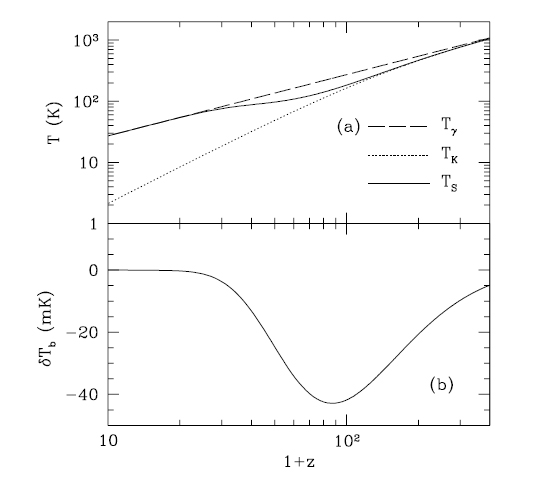
\includegraphics[width=0.95\linewidth]{Introduction/figures/dark_ages_global_spectrum.jpg}
\caption{(a) Plot of $T_S$, $T_\gamma$, and $T_K$ during the dark ages and (b) $\delta T_b$ during the same period given only collisional coupling from furlanetto et. al. \cite{furlanetto_2006}}
\label{Fig:da_global}
\end{center}
\end{figure}

\subsubsection{Dark Ages}
During the dark ages, the universe expanded at a rate defined by the Hubble parameter. Initially, the IGM was dense enough for Compton scattering between CMB photons and free electrons in the IGM to set \tk$=$\tg. But as the gas adiabatically expanded, thermal decoupling caused \tk to decrease. At this time, collisions between baryons in the IGM kept $x_K$ large, so that the spin temperature decreased below the CMB temperature. 

However, this coupling gradually decreased as the rate of collisions between baryons decreased, and the spin temperature increased back to match the CMB temperature. The process of cooling and decoupling created a dip in \ts, which most models predict should be centered around $z \sim 80 $ \cite{furlanetto_2006}. Figure \ref{Fig:da_global} shows one model prediction for the relevant temperatures including \tg, \tk, \ts and \dtb before star formation. 

At the same time, the first generation of stars began to form in the overdense regions of space. 

\subsubsection{Formation of the First Stars}

\textcolor{blue}{Need to add discussion of first stars.}

\begin{figure}[htb]
\begin{center}
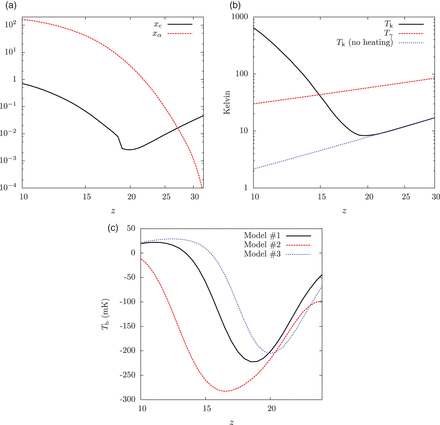
\includegraphics[width=0.95\linewidth]{Introduction/figures/ts_evolution.png}
\caption{Plots of (a) $x_K$ and $x_{\alpha}$, (b) $T_\gamma$ and $T_K$ with or without x-ray heating, and (c) $\delta T_b$ during the Cosmic Dawn for different models of star formation from natarajan et. al. \cite{natarajan_2014}}
\label{Fig:cd_global}
\end{center}
\end{figure}

\subsubsection{Cosmic Dawn}
With the birth of the first stars, light began to propogate through the IGM. This light included \lya photons, which re-coupled \ts and \tk via the Wouthuysen-Field mechanism. Since the kinetic temperature of the IGM was at this point much lower than \tg, this re-coupling decreased \ts. 

Meanwhile, x-ray photons were produced by two types of sources among the first Pop.III stars. One source was electrons accelerated by supernovae to relativistic speeds. When these electrons undergo inverse Compton scattering, x-ray photons are produced. The other source was high-mass x-ray binary stars, which occur when massive stars on the main sequence lose material through accretion onto a compact neighbor such as a neutron star, black hole or white dwarf star. 

These high energy photons heated the IGM through a combination of photoionization of Hydrogen or Helium and collisions with IGM components \cite{furlanetto_2006}. 

Depending on the rate of x-ray heating compared to the rate of \lya coupling, the spin temperature is predicted to dip during the period where $x_k>0$ and \tk is less than \tg. By varying the model of first star formation, the exact shape of the dip in the spin temperature can be adjusted. Most models predict a dip centered around $z\sim20$, with a width of $0 \leq z \leq 10$ and a depth of $0\leq \Delta T \leq 300 mK$. Figure \ref{Fig:cd_global} shows a few models of global \dtb during the Cosmic Dawn, as well as some of the parameters that feed into the brightness temperature variance. 

\textcolor{red}{Add figure here to show reionization.}

\subsubsection{Epoch of Reionization (EoR)}
As the kinetic temperature of the gas continued to rise, it reached the threshold where Equation \ref{Eq:dT_b} breaks down because the kinetic and spin temperatures of the gas are large enough that the approximation used for \tu is no longer applicable. At this point \dtb reaches a maximum. Meanwhile, the propogation of x-ray photons through the IGM also began to ionize the hydrogen atoms. Since the brightness temperature of the \cm signal is also proportional to the amount of neutral hydrogen ($x_{HI}$) present in the IGM, as shown in Equation \ref{Eq:dT_b}, this ionization process caused a gradual decrease in the average \cm signal. 

\subsection{Era of Acceleration}
In the modern universe post reionization, neutral Hydrogen gas in the IGM is limited to the regions around galaxies. This gas can still be mapped using the \cm signal, but the magnitude of the signal is much smaller than in previous eras. 

\textcolor{red}{Not sure how much science detail to include about the era of acceleration since it's not the main focus of the rest of the thesis.}

\textcolor{red}{Add figure here to show \cm signal as a function of frequency or make sure that the previous figures include frequency information.}

\section{Measuring the \cm Signal}
After passing through the IGM at a given time, the \cm photons travel toward the earth. As they travel, the photons frequencies are redshifted ($\nu_{meas} = \nu_{10}/(1+z)$) from their original frequencies. This shift allows us to measure a spectrum $\delta T_b (\nu)$, where $\nu$ is the frequency at which the signal is measured, corresponding to the redshift where the signal was produced. 

Measurements of the \cm spectrum are classified in two types. The first type aremeasurements of the sky-averaged spectrum \avgdtb, while the second type are measurements of the fluctuations in the \cm spectrum ($\delta_{T_b} =  \delta T_b (\nu)/ T_b (\nu)$) using the power spectrum of the fluctuations ($ \tilde{ \delta_{T_b} } ( \vec{k} )$) \cite{natarajan_2014}. 

\begin{figure}[htb]
\begin{center}
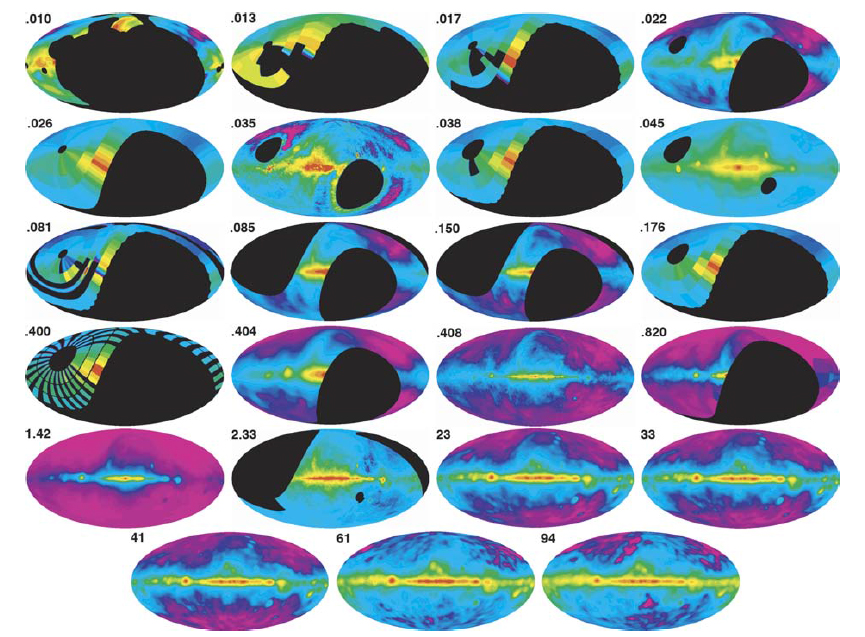
\includegraphics[width=0.95\linewidth]{Introduction/figures/GSM_maps.jpg}
\caption{Plots of radio sky measurements used to construct the Global Sky Model \cite{GSM_model} of radio foregrounds. The number in the upper left corner of each plot is the frequency (in GHz) at which the map data was collected, while the color scale is the log of the sky temperature in Kelvin.}
\label{Fig:GSM_maps}
\end{center}
\end{figure}

\subsection{Foregrounds}
One of the greatest challenges of making any \cm measurements is the presence of foregrounds in the data. These foregrounds include any signals on the sky that aren't related to the CMB brightness temperature (\tb) and its variance due to the IGM. Foreground signals come from astrophysical sources which emit in the low frequency radio band ($\nu \leq \nu_{10}$), interference from Earth's ionosphere, and radio frequency interference (RFI) from man-made sources. We will discuss RFI in Chapter \ref{Ch:RFI} and ionospheric impacts in Chapter \ref{Ch:Iono}, so in this section I will focus on astrophysical foregrounds. 

For $\nu \leq \nu_{10}$ the dominant astrophysical foreground is synchrotron radiation from the Milky Way Galaxy. This radiation comes from free electrons in the galaxy and has a strongly sloping spectrum \cite{furlanetto_2006}, as shown in Equation \ref{Eq:T_sky}. 

\begin{equation}\label{Eq:T_sky}
T_{sky} \approx 180 \Big( \frac{\nu}{180 MHz} \Big)^{-2.6} K
\end{equation}

Maps of the astrophysical foregrounds have been made at a number of frequencies, including the $''$Haslam$''$ map at 408 MHz and the WMAP maps (after removal of the CMB signal) at 23,33,41,61 and 94 GHz. These maps are shown in Figure \ref{Fig:GSM_maps}. A model of the foregrounds from $10 MHz-100 GHz$ was constructed using the maps, as outlined in de Oliveira-Costa et al \cite{GSM_model}. This sky model is commonly used for foreground assessment and even calibration by \cm experiments. A discussion of how the model is used in one particular application can be found in Section \ref{Sec:GSM}. 

\subsection{Average (Global) \cm Frequency Spectrum (\avgdtb)}
In order to make a measurement of \avgdtb, experiments need to be designed that measure the total sky brightness temperature spectrum ($T_{Sky}$) over a wide range of frequencies. These experiments will measure the combination of signals collected by an antenna:

\begin{equation}
T_{ant} = T_{fg} + T_b +T_{sys}+T_{RFI} = T_{Sky} + T_{sys}
\end{equation}

where $T_{fg}$ is the astrophysical foreground signal, $T_{RFI}$ is the man-made signal, $T_{sys}$ is the system temperature, and \tb is the brightness temperature from the CMB. The system temperature $T_{sys}$ will be a combination of thermal noise and instrument noise. Thermal noise is set by the radiometer equation ($T_{thermal} = T_{ant}/\sqrt{BW \tau}$), where $BW$ is the system bandwidth and $\tau$ is the integration time \cite{carroll2007}. Instrument noise comes from the electronics in the system (such as the amplifiers). 

Extracting the \cm brightness temperature spectrum requires removing all of the other terms in the data. Different strategies have been proposed for removing these signals, but all of them rely on the fact that the other signals have a different type of spectral structure than the \cm signal. We will discuss one such strategy for foreground removal in a \avgdtb experiment in Chapter \ref{Ch:Data}.

\subsection{\cm Fluctuation Power Spectrum}
Like the \avgdtb experiments, power spectrum measurements will also be dominated by foregrounds. 

\textcolor{red}{Not sure how much detail to put here since it's not directly relevant to the science discussed in the rest of the thesis.}


\section{\cm Experiments}
There are a number of experiments specifically designed to measure the \cm global signal or power spectrum. These experiments are either currently gathering data or are still under development. Preliminary constraints on the \cm signals have been placed for different cosmological eras, and future measurements should continue to tighten those constraints such that we will have a good detection of the \cm global signal and power spectrum during the Dark Ages, Cosmic Dawn, Epoch of Reionization and Era of Acceleration. 

\subsection{Global Experiments}
There are a number of experiments trying to measure the \avgdtb signal during different cosmological eras. These experiments focus on redshifts where \dtb is large and/or has a large first derivative. EDGES \cite{bowman_2008} is a single antenna system focused on frequencies $100-200 MHz$, and has placed upper limits on the signal during the Epoch of Reionization. 

LEDA \cite{leda}\cite{bernardi_2014} and DARE \cite{burns_2011} are currently under development, and are targeting the Dark Ages and Cosmic Dawn. LEDA is designed to operate on the ground using a combination of an interferometer and a single antenna, while DARE intends to launch a satellite in orbit around the moon with a single antenna. 

Both of these experiments have large budgets of over \$ 1 million dollars and require significant resources and technology development. In contrast, the EDGES experiment is on a much smaller scale and can be deployed in the field with minimal infrastructure. 

\subsubsection{SCI-HI Experiment}
We were inspired by the EDGES experiment to develop a similar system focusing on a different part of the \cm spectrum ($40 \leq \nu \leq 130 MHz$) and going after the Cosmic Dawn signal. This experiment is the SCI-HI experiment, and will be the main focus of the rest of this thesis. Chapter \ref{Ch:System} details the experiment design, chapter \ref{Ch:RFI} discusses the search for an experiment site, chapter \ref{Ch:Data} details the data analysis done on data collected with the experiment in June 2013, and chapter \ref{Ch:Conclude} outlines the plans for the continuation for the SCI-HI project. 

\subsection{Mapping Experiments}
Experiments which seek to measure the \cm power spectrum are typically many-element interferometers, each with a different antenna design and configuration. Early projects, including the GMRT-EoR \cite{paciga_2013} project, made use of existing telescopes to make measurements. Meanwhile, a number of projects were designed and constructed such as the Precision Array for Probing the Epoch of Reionization (PAPER) \cite{pober_2013}\cite{jacobs_2014}, the Murchison Widefield Array (MWA) \cite{bernardi_2013}\cite{tingay_2012}, and the Low Frequency Array for Radio Astronomy (LOFAR) \cite{jelic_2014}\cite{lofar}. These projects have put first constraints on the power spectrum during the Epoch of Reionization. 

Future projects targeting the Epoch of Reionization signal include the Hydrogen Epoch of Reionization (HERA) \cite{hera}\cite{bernardi_2014} array and the Square Kilometer Array (SKA) \cite{ska}.

Beyond the EoR projects, there are a number of power spectrum projects focusing on lower redshifts during the Era of Acceleration. The \cm signal targeted by these projects is much smaller than the EoR signal, but the foregrounds at these frequencies are also much smaller. First constraints on the power spectrum were placed by the GBT-IM project \cite{masui_2012}\cite{switzer_2013}, which used the Green Bank Telescope to make a map of a few degree patch of sky and construct a power spectrum from that map. 

Like with the EoR experiments, full sky mapping requires a dedicated project. One such project is the Canadian Hydrogen Intensity Mapping Experiment (CHIME) \cite{shaw_2014}\cite{chime}, currently under development. CHIME uses a unique cylindrical interferometer design to map the sky. 

Chapter \ref{Ch:Planet} includes some discussion of the Green Bank Telescope and CHIME, and how they were used in a public outreach project for educating the public on \cm observations. 

